%%%%%%%%%%%%%%%%%%%% author.tex %%%%%%%%%%%%%%%%%%%%%%%%%%%%%%%%%%%
%
%%%%%%%%%%%%%%%% Springer %%%%%%%%%%%%%%%%%%%%%%%%%%%%%%%%%%

\title*{A detailed analysis of a PushGP run}
% Use \titlerunning{Short Title} for an abbreviated version of
% your contribution title if the original one is too long
\author{Nicholas Freitag McPhee, Maggie M. Casale, Mitchell D. Finzel, Thomas Helmuth and Lee Spector}
\authorrunning{McPhee, Casale, Finzel, Helmuth, and Spector}
% Use \authorrunning{Short Title} for an abbreviated version of
% your contribution title if the original one is too long
\institute{Nicholas Freitag McPhee, Maggie M. Casale and Mitchell D. Finzel \at University of Minnesota, Morris; Morris, MN USA
\and Thomas Helmuth \at Washington and Lee University, Lexington, VA USA
\and Lee Spector \at Hampshire College, Amerherst, MA USA}

\maketitle

\abstract{We analyze the key events in a GP run!}

\begin{keywords}
	genetic programming, PushGP, ancestry graph, lineage, inheritance
\end{keywords}
\index{genetic programming}
\index{PushGP}
\index{ancestry graph}
\index{lineage}
\index{inheritance}
\\
\section{Introduction}
\label{sec:introduction}

\todo{Scrape some citations from the VizGEC 2016 paper.}

Previous work~\citep{McPhee:2015:GPTP, donatuccianalysis, Burlacu:2013:GECCOcomp:new, Burlacu:CIEES:2015, kuber2014ancestral} has
illustrated the value of ancestry graphs as a means of analyzing the dynamics
of evolutionary computation runs. In~\cite{McPhee:2015:GPTP}, for example, we
demonstrated the use of graph databases as a tool for collecting and analyzing
ancestries in genetic programming runs, identifying several key moments and
general patterns in runs using both lexicase and tournament selection.

In this paper we extend that work to provide a more detailed analysis of a
single, complete run. We identify \emph{every} ancestor of the evolved 
solutions, and
then reduce that graph (which has 394 individuals) to a graph containing only 
the individuals that in fact contributed one of the key instructions to 
the final solutions (73 individuals). We then trace each of these key solution
instructions back through the entire lineage, identifying where they were first
introduced, and how they were transmitted through the genetic history. This
reveals a number of interesting properties of this particular run including,
for example, the fact that 4 of the 9 key instructions were introduced via 
mutation.

In Section~\ref{sec:background} we review the key components of the system
used to generate the run explored here (PushGP, Plush genomes, and the Replace Space With Newline test problem). We then describe and present both the full
and filtered ancestry graphs in Section~\ref{sec:ancestryGraphs}, before
tracing the evolutionary history of all the key instructions in 
Section~\ref{sec:howDidWeGetThere}. Our discussion in 
Section~\ref{sec:discussion} builds on the details of these traces and
catalogues the kinds of events we see in this run, describing a few in greater
detail. We then wrap up with some conclusions and ideas for future work in
Section~\ref{sec:conclusions}.

\section{Tools and setup}
\label{sec:background}

The run presented here uses the PushGP genetic programming system, which evolves programs in the Push programming language \citep{spector:2002:GPEM, 1068292}. Push programs use multiple typed stacks to store and manipulate data. Instructions take their arguments from stacks of the appropriate types and leave their results on the appropriate stacks. Push provides support for iteration, recursion, conditional execution, and automatically-defined subroutines through runtime code manipulation, making it a Turing-complete language \citep{1068292}. PushGP implementations have been written in Clojure, C++, Java, JavaScript, Python, and others. Many of these are available from the Push project page.\footnote{\url{http://pushlanguage.org/}} The run presented here was conducted using the Clojure implementation of PushGP\footnote{Clojush: \url{https://github.com/lspector/Clojush}}.

Push gains much of its power as an evolutionary language from its ability to manipulate code, including the currently executing code, as a program runs. The running program is stored on the \textit{exec} stack, allowing instructions to change code before it runs. Push programs are hierarchically structured into code blocks delimited by parentheses. Each code block acts as a single unit when code manipulating instructions act on them. For example, the \texttt{exec\_if} instruction deletes the second code block on the \texttt{exec} stack if the top item on the \texttt{boolean} stack is true, and deletes the first code block on the \texttt{exec} stack if it is false.

Unlike previous versions of PushGP, Clojush has recently been changed to not evolve 
Push programs directly, but instead uses a new linear genome representation 
\citep{Helmuth:2016:GPTP}. Each \textit{Plush genome}\footnote{\textbf{L}inear 
	\textbf{Push}} consists of a linear sequence of instructions (including 
literals), and is translated into a Push program prior to execution. Each 
instruction may have one or more epigenetic markers attached that modify how 
the genome is translated into a Push program.
%For example, the \textit{silent} marker is a boolean that tells whether a 
%particular instruction will appear in the translated program. 

Most relevant to this study is the \textit{close} epigenetic marker, which 
affects the hierarchical composition of programs. Since many Push instructions 
do not take arguments, as in code blocks, from the \textit{exec} stack, it 
makes sense to limit the appearance of code blocks to follow only instructions 
that make use of them. Each instruction that takes one or more argument from 
the \textit{exec} stack automatically opens one or more code blocks. Then, the 
integer close marker attached to each instruction tells how many opened code 
blocks to close after the instruction. During translation from Plush genome to 
Push program, an open parenthesis is placed after each instruction that 
requires a code block, and a matching closing parenthesis is placed after a 
later instruction with a non-zero close marker. These code blocks can create 
hierarchically nested Push programs, allowing, for example, structures such as 
nested looping and subroutines containing conditional code.

The use of linear genomes allows PushGP to use simple uniform genetic 
operators. The operators used in this study are inspired by the operator ULTRA. 
ULTRA, designed for use on Push programs, requires programs to be translated 
into a linear form and back \citep{Spector:2013:GPTP}, potentially requiring 
repair of the program. Our main crossover operator, \textit{alternation}, 
traverses two parents in parallel while copying instructions from one parent or 
the other to the child.

%While traversing the parents, copying can jump from one parent to the other with probability specified by the \textit{alternation rate} parameter. When alternating between parents, the index at which to continue copying may be offset backward or forward some amount based on a random sample from a normal distribution with mean 0 and standard deviation set by the \textit{alignment deviation} parameter.

We also use a \textit{uniform mutation} operator that traverses a parent, 
replacing each instruction with some small probability. Similarly, a 
\textit{uniform close mutation} operator can change the close epigenetic marker 
attached to an instruction by incrementing or decrementing it. Finally, we 
often apply an alternation operator followed by a uniform mutation of the 
result, inspired by the ULTRA operator \citep{Spector:2013:GPTP}.

Push also implements a method of automatic simplification, which takes a program and 
converts it into a smaller, semantically equivalent program. This process uses 
hill-climbing to remove instructions and code blocks from the program, checking 
at each step that the resulting program produces the same error vector as the 
original program \citep{Spector:2014:GECCOcomp}.

Our goal here is to give a deep analysis of a single run of PushGP, exploring and analyzing many of the programs, selections, and variations that make up this run. We chose to analyze a run on the Replace Space With Newline (RSWN) problem, taken from a recent general program synthesis benchmark suite \citep{Helmuth:2015:GECCO}. In this problem, a program is given a string as input and should perform two tasks: first, it must print the result of replacing each space in the input with a newline character, and second, it must functionally return the number of non-whitespace characters in the input. Push functionally returns values by taking them from the top of relevant stacks. For example, each program evolved in this run returns the top integer on the integer stack as its output, unless the stack is empty. We include instructions that allow programs to print literals to standard output.

\todo{Say that we're using Titan and Graphviz for all this.}

%\subsection{THIS COPIED FROM TOM'S THESIS}

%% I (Tom) left the following in the tex in case we need more info later; most of it isn't represented above. If we use it, it shouldn't be copied directly as to not plagiarize Tom's thesis.

% Push dedicates a separate stack for each data type. Instructions take their arguments from stacks of the appropriate types and they leave their results on stacks of the appropriate types. This allows instructions and literals to be freely intermixed regardless of type while still ensuring execution safety. The convention in Push regarding instructions that are executed in contexts that provide insufficient arguments on the relevant stacks is that these instructions act as ``no-ops''; that is, they do nothing.

%Push traditionally takes results from the top items on stacks after executing a program. For example, a program that returns an integer will take the top value on the integer stack as its output. This convention means that some evolved programs might not return a value of the correct type, if the relevant stack is empty following execution; in this scenario, we penalize the program for failing to return a result. Push also has the ability to print literals to standard output; in our implementation this simply concatenates printed material to a string of whatever has been printed so far, but this could easily be changed to print to standard output.


\section{Ancestry graphs}
\label{sec:ancestryGraphs}





\begin{itemize}
	\item Describe the basics of the run (length, etc.).
\end{itemize}

Then work backwards from the winner back through to the start of the run.

\subsection{Full ancestry graph}

Figure~\ref{fig:run0Labelled} shows the full ancestry tree of the 13 successful 
individuals in this run. Each individual in the run is represented with a
rectangle containing an identifier of the form \texttt{X:Y}, where \texttt{X}
is the generation number, and \texttt{Y} is an arbitrary individual number
within that generation. Each generation is a row, with the initial random
individuals being at the top and the 13 successful individuals at the bottom.

\begin{sidewaysfigure}[tb!p] %[b] sets the image at the bottom of the page; t = top, b = bottom, h = here%
	% \sidecaption
	% Use the relevant command for your figure-insertion program
	% to insert the figure file.
	% For example, with the graphicx style use
	\begin{center}
		\vspace{0.6\columnwidth}
		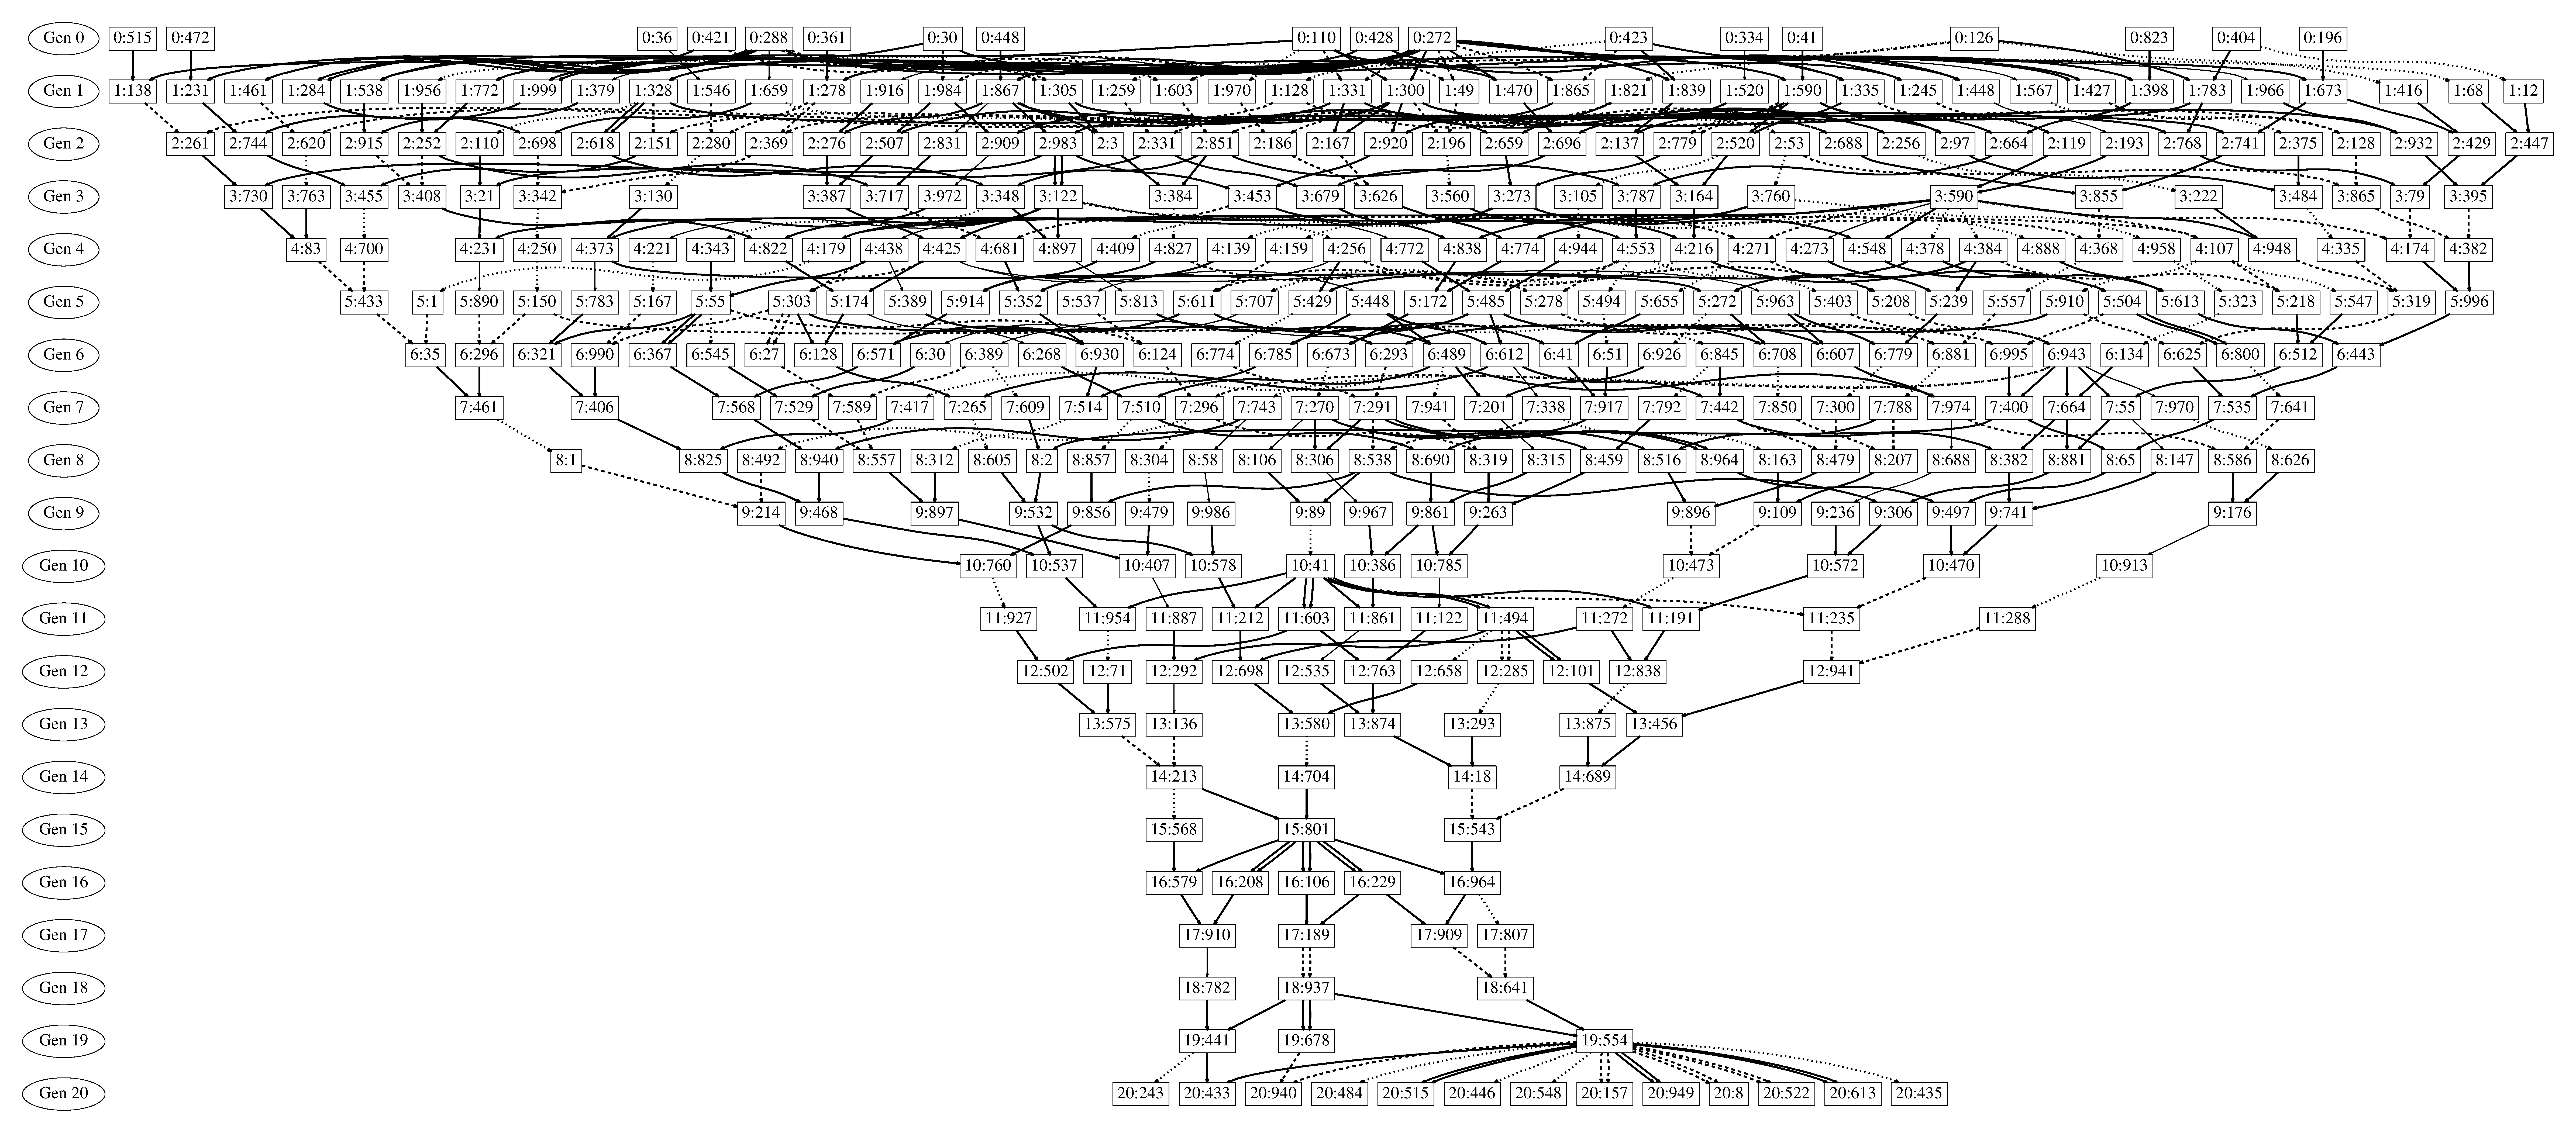
\includegraphics[width=\columnwidth]{../figures/run0_GPTP_2_font_30}
	\end{center}
	\caption{The labelled run.}
	\label{fig:run0Labelled}       % Give a unique label
\end{sidewaysfigure}

The edges indicate the particular genetic operator used to construct a child
as follows:
\begin{itemize}
	\item Dashed: alternation
	\item Dotted: uniform mutation
	\item Thin black lines: uniform close mutation
	\item Thick black lines: alternation and uniform mutation
\end{itemize}

This graph includes \emph{every} individual in this run that was an 
ancestor of one of the winners, i.e., every individual that could possibly have 
contributed genetic material to one of the winners. Note, however, that not
all these individuals actually contributed any genetic material to those
solutions. There are, for example, cases where one of the parents actually
contributed no material in a recombination (alternation) event, and cases where
a parent did contribute some genetic material, but that material was later
removed or replaced in subsequent mutations or recombinations. 

Conversely, while the individuals not represented in this graph are
guaranteed to have not contributed to the genetics of the successful
individual, they might have still had some substantial impact on the
run's overall dynamics. The presence of those individuals and their
error vectors could certainly affect lexicase selection's choice of parents,
for example, which could substantially impact the dynamics.

\subsection{Filtered ancestry graph}

Despite the short length of this run, and the restriction to just displaying
ancestors of successful individuals, Figure~\ref{fig:run0Labelled} still
contains 394 nodes and 629 edges, making it difficult to analyze in full.
Figure~\ref{fig:run0Filtered} is a version of the same graph that further
filters the ancestry tree, attempting to highlight the individuals that
are most likely to have contributed a significant amount of genetic material
to the solutions.

\begin{figure}[tb!p] %[b] sets the image at the bottom of the page; t = top, b = bottom, h = here%
	% \sidecaption
	% Use the relevant command for your figure-insertion program
	% to insert the figure file.
	% For example, with the graphicx style use
	\begin{center}
		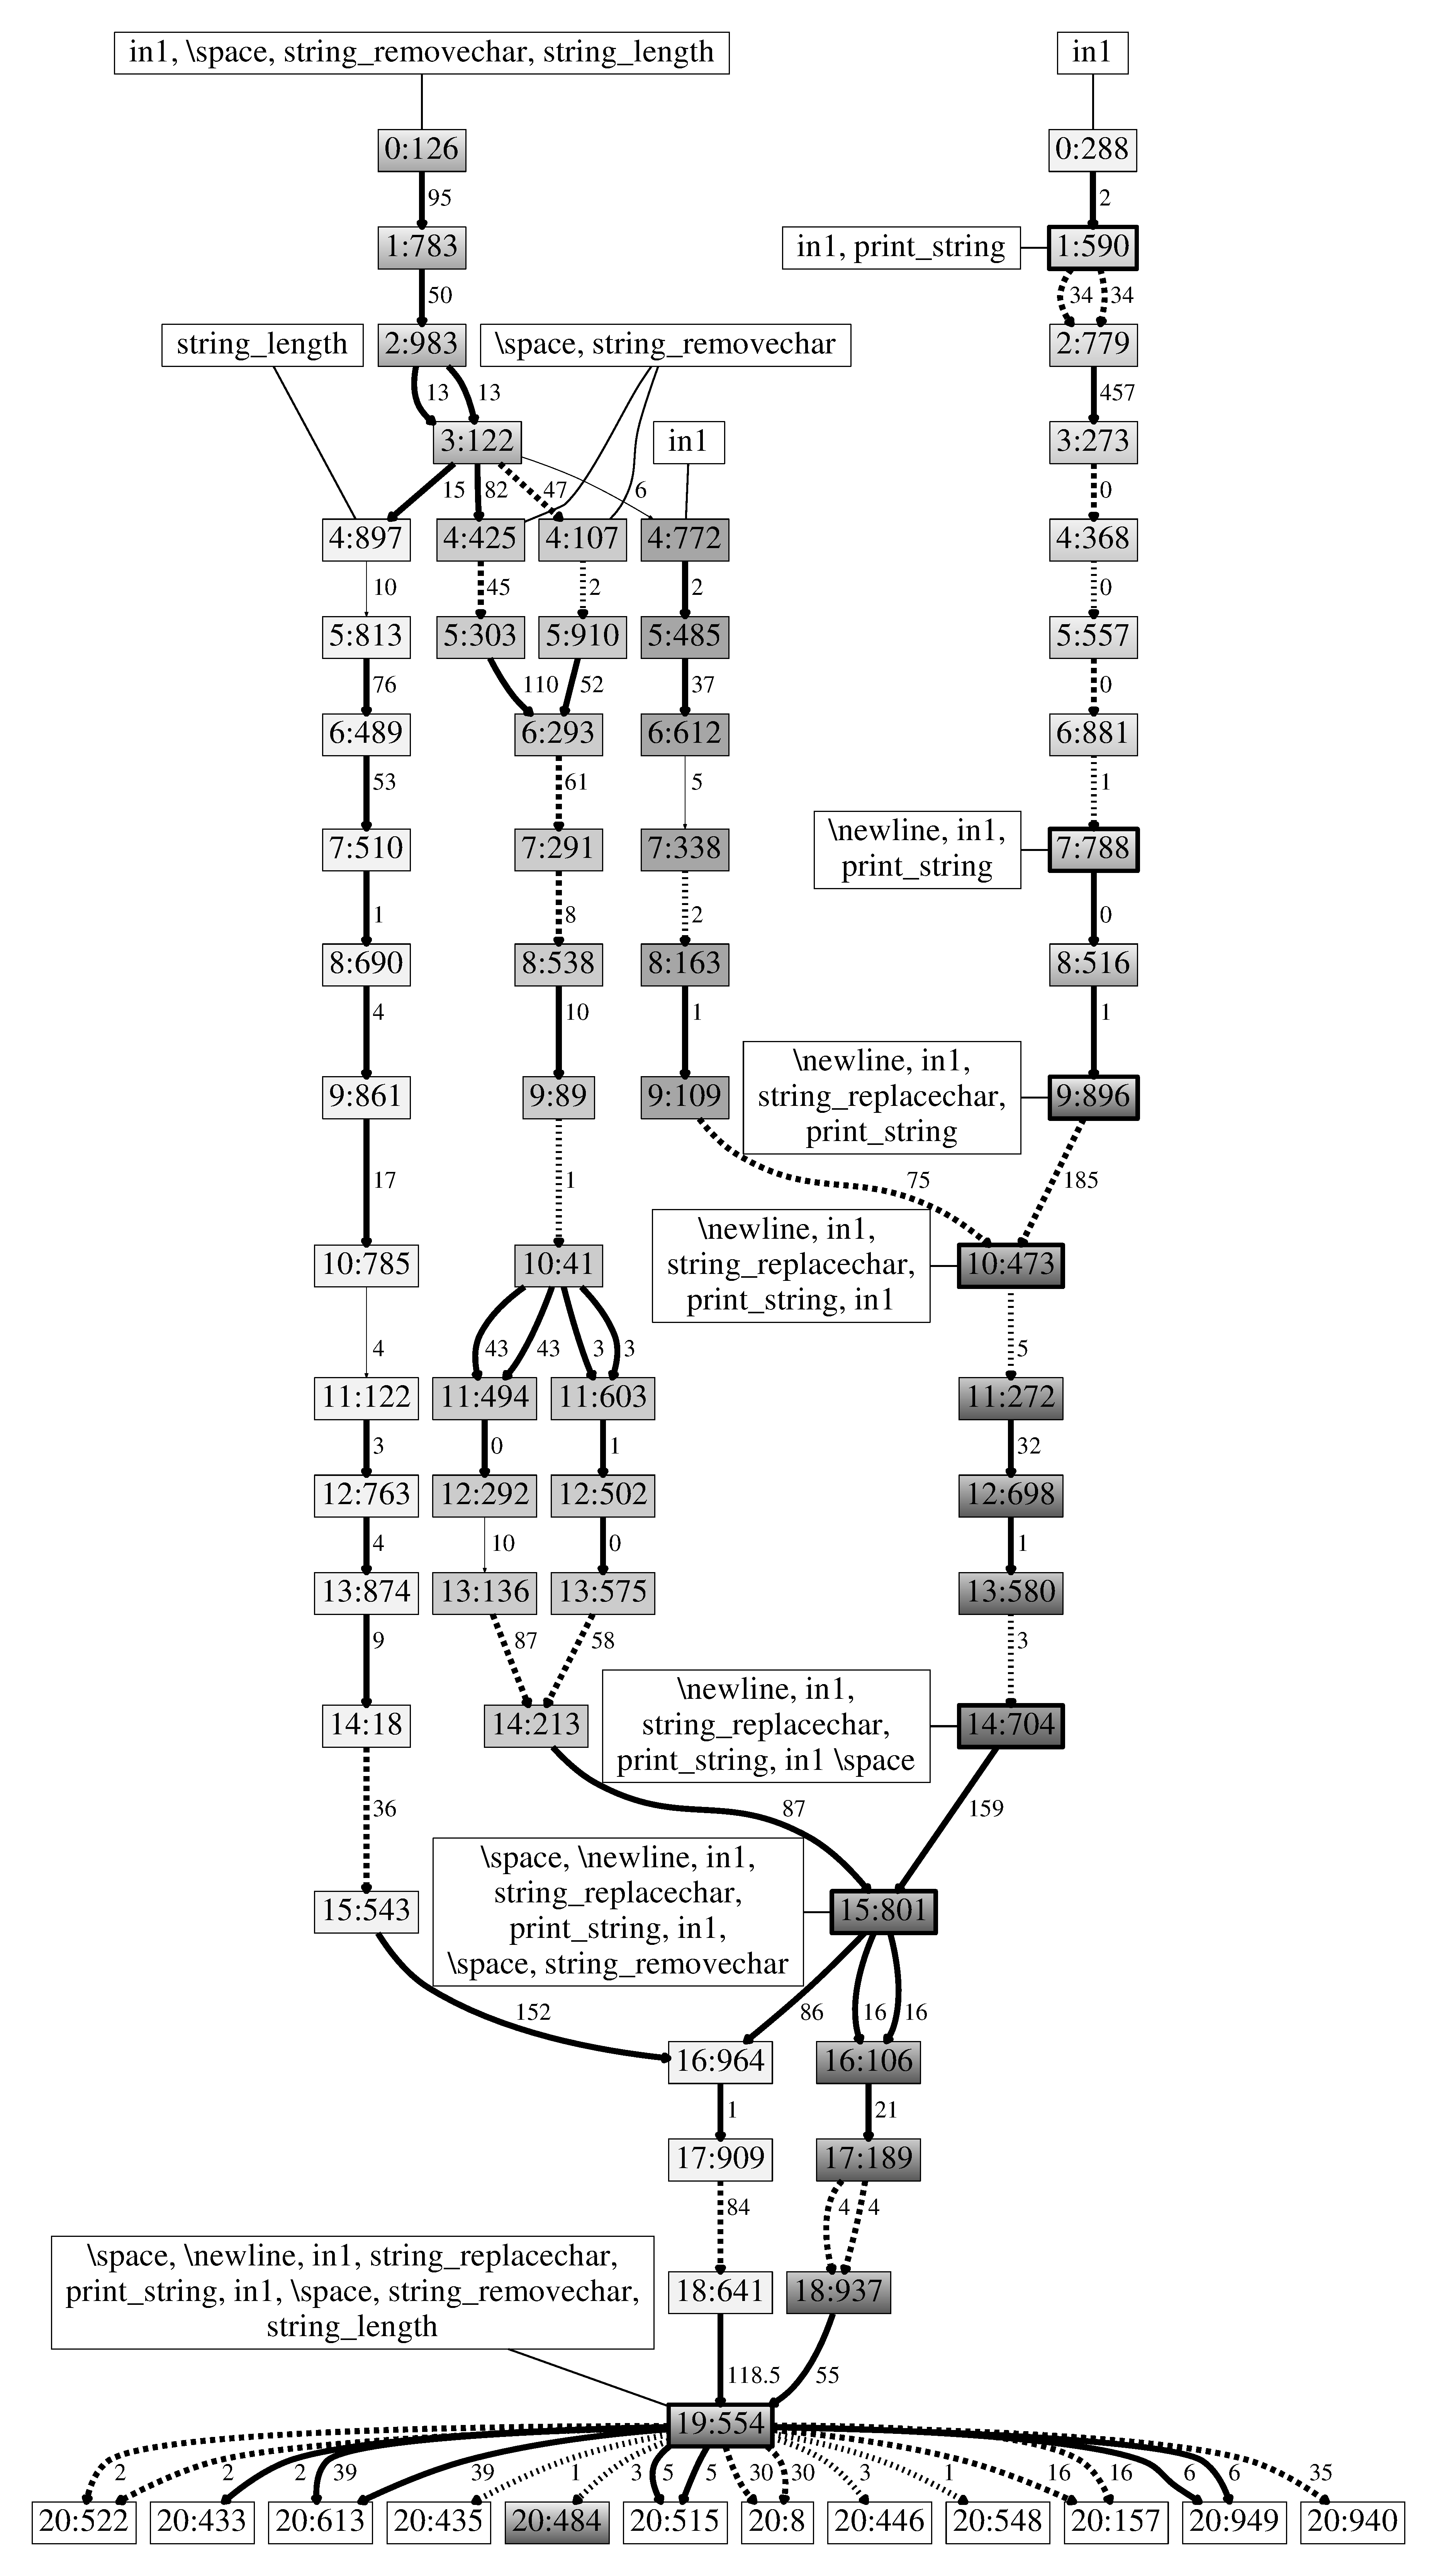
\includegraphics[height=\textheight]{../figures/filtered_fill}
	\end{center}
	\caption{The filtered version of the run's ancestry graph.}
	\label{fig:run0Filtered}       % Give a unique label
\end{figure}

We implemented this filtering by first computing the Damerau-Levenshtein 
distance (DL-distance)
between genome vectors for each parent-child pair; these distances
are indicated as edge labels in Figure~\ref{fig:run0Filtered}. The genome
vectors were generated by extracting the \texttt{:instruction} and 
\texttt{:close} fields from each gene, and concatenating those into a
single sequence. So, for example, the genome of successful individual
20:484 starts

\todo{Should this prefix of the genome be in a figure so it doesn't
	get broken up by things like page breaks?}
\begin{verbatim}
	{:instruction boolean_and, :close 0} 
	{:instruction boolean_shove, :close 0} 
	{:instruction exec_do*count, :close 0} 
	{:instruction exec_swap, :close 0} 
	{:instruction integer_empty, :close 0}
	...
\end{verbatim}

making the associated genome vector

\begin{verbatim}
	boolean_and 0 boolean_shove 0 exec_do*count 0 
	   exec_swap 0 integer_empty 0 ...
\end{verbatim}

\todo{Replace the filtering stuff with a description of how Figure~\ref{fig:run0Filtered} was generated.}

Once we had these distances computed, we used it to identify parents in
recombinations that made minimal contributions to the resulting child, so
we could avoid tracing back through those edges, potentially removing not
just that parent, but it's parents, grand-parents, etc. 

The logic for this filtering was fairly straightforward, even simplistic.
First assume we have two parents, $p$ and $q$, and a child $c$ such that:
\begin{align*}
	a & = \textrm{DL-distance}(p, c) \\
	b & = \textrm{DL-distance}(q, c) \\
	s & = \textrm{genome-length}(c)
\end{align*}
and assume without loss of generality that $a \leq b$ (i.e., $p$ is the
closer parent). Then we filtered out parent $q$ if either:
\[
	(a < 0.2 \times s) \lor (b \geq 2 \times a).
\]
Thus parent $q$ will be filtered out if parent $p$ is particularly close to
the child, or if parent $q$ is more than twice as far away from the child as
parent $p$. The choices of the constants $0.2$ and $2$ are obviously somewhat
arbitrary, but appeared to work reasonably well on a variety of datasets. 
There are,
however, examples where a filtered parent did in fact contribute a significant
number of instructions to the offspring, so one would need to be careful in not
making overly broad assumptions based on an individual not being in the filtered
version of a graph.

A notable consequence of this filtering is that many of the larger DL distances in
the filtered graph are the product of there being a child with both parents present.
For instance when 13:575 and 13:136 converge into 14:213 they have DL distances of
58 and 87 respectively. While an alternation with uniform mutation and one parent present,
such as 8:163 into 9:109,  only has a DL distance of 1.

\subsection{The (successful) end}
\label{sec:successfulEnd}

\todo{I think this should probably move down to the next section? -- NFM}

There are 13 successful individuals
in this run, most of which have identical simplified
programs. In the interest of space we're going to focus on one of those, 
individual 20:484, which was constructed via three instruction mutations
from individual 19:554.
Individual 20:484's genome contains 194 genes, and the unsimplified 
program also contains 194 instructions and has zero error on both
the training and testing cases.
The simplified program for 20:484 (which also passes all the tests)
contains only 9 instructions:
\begin{verbatim}
(\space \newline in1 string_replacechar print_string
 in1 \space string_removechar string_length)
\end{verbatim}
This simplified program is actually quite readable, and has a similar
structure to what me might expect from a human solution.
The first five 
instructions (together on the first line) replace all the spaces in the input string 
with newlines (using the \texttt{string\_replacechar} instruction) and print the 
resulting string, thereby solving half the problem. 
The next four instructions (on the second line) remove all the spaces from
a fresh copy of the input string, compute the length and leave that on the
\texttt{:integer} stack as the ``returned'' result.

\section{How did we get there?}
\label{sec:howDidWeGetThere}

In this section we will trace the origin of each of the nine instructions
in the simplified program for individual 20:484,
going back to their introduction either via a mutation or as an element 
of one of the initial, random programs in the initial generation. It's clear
that each of these was ``necessary'' for the construction of this particular
solution, so knowing where they all came from and how they came together
should give us a valuable sense of the dynamics of this run. 

It's important to realize, however, that this will
never be the whole story. Push instructions and values can play an 
important role in subtle ways, e.g., as spacers on stacks that when
``counting'' is implemented with a stack depth command. Removal of
instructions can also be important. One key step in this run, for example, 
is the removal of an extraneous \texttt{print\_newline}; the presence of this
instruction caused the printed output to always have an error of one,
and its removal led to 100 errors changing
from 1 to 0. All that said, however, we need some way to limit the number
of individuals and events to analyze, so here will focus on the how those
nine instructions trace through the ancestry.

It's also important to note that we didn't actually collect enough information
to \emph{always} say for certain where an instruction came from in a 
recombination event. There are numerous copies of instructions like
\texttt{in1} in most of the genomes, for example, and in principle any of them
in a parent could be the source of an \texttt{in1} in the child. In practice,
however, there are constrains of location and order that typically allowed
us to identify a single, unique source. There were a few places, however, where
judgement calls were made. In future work we're going to explore attaching
unique IDs to each gene and track not just parent-child relationships, but
also source-destination relationships among genes, as this will give us
certainty about the sources of genes, and allow us to automate more of the
analysis, all at the expense of larger databases.

Returning to the specific program from Section~\ref{sec:successfulEnd},
it turns
out that the evolution of the first five instructions, those handling the
printing part of Replace Space With Newline, is largely independent of
the evolution of the last four instructions, which handle the return part
of the problem. The first five instructions, for example, all appear early 
in the genome for 20:484, from gene 9 to gene 24, while the last four 
all appear much later in the genome, from gene 107 to gene 175. As a consequence
we'll trace these two groups one at a time.

\subsection{Printing: The first five instructions}
\label{sec:Printing}

What is witnessed in the ancestry of the 5 instructions key to solving the printing test
cases (even cases) is fairly interesting and straightforward. Starting at the top with individual 0:288 only
one of the key instructions, \texttt{in1}, is present. The rest of the 5 are introduced over time purely
through uniform mutations. The next of the key instructions to appear is introduced in individual 1:590 via a point
mutation converting a piece pf 0:288's genome into a \texttt{print\_string} instruction. These two
instructions are passed along this tree until they are joined by the next important instruction,
\texttt{\textbackslash newline}. This instruction is introduced in 7:788 via a uniform mutation
of 6:881.

After descending another 2 generations these three instructions were joined by \texttt{string\_replacechar}
in 9:896 via yet another uniform mutation. At this point it's interesting to note that these instructions are
all introduced fairly evenly over the course of these generations. Even as the run gets closer to the generation
20 winners these individuals obtained key instructions through random uniform mutations. Which lead to
the final of these key instructions being introduced, \texttt{\textbackslash space}.
This instruction is added in generation 14 via a uniform mutation of 13:580 into 14:704, thus completing the five key printing
instructions that are passed down through 15:801 and maintained all of the way down to the winners.

This marks another interesting point about these instructions. Unlike in the return case instructions there is a 
very clear and straight path of lineage for these instructions. As they are introduced over time they 
are never split apart into subtrees to be recombined later. Rather they were added via mutation and 
then passed down together consistently from 0:288 down to the winners.

These instruction additions can also be seen affecting the error vectors in their individuals. Each instruction is addition
is accompanied by a shift in the even test cases. Sometimes it is a small effect with both positive and negative change
to the test cases, but others it is a more dramatic improvement. For instance an example of a small change is when
\texttt{\printindex\_string} is mutated into 1:590. With this mutation we saw a change in 83 of the 100 even test cases
with general improvements across the board accompanied by a few increases in test scores (performed worse). Meanwhile in
the mutation of 13:580  in the creation of 14:704 we saw all of the even test scores become 1. This is in general a very
big improvement, but worsened a few tests that had passed with no error in 13:580. These examples help to highlight
and support the value of these instructions as each step we saw a change, mostly for the better. This however is not to
say that steps where these instructions are not added don't haven't had changes in their error vectors, but shines light
on how it is necessary to both find the right instructions as well as remove instructions that hinder the solution.

\subsection{Returning: The last four instructions}
\label{sec:Returning}

These last four instructions were present in the right order and in at least
rough proximity in the very first generation, in individual 0:126. The first of these instructions (\texttt{in1}) was on gene 75 of the genome, the next two
(\texttt{\textbackslash space} and \texttt{string\_removechar}) were on 
genes 89 and 94, and then the final instruction (\texttt{string\_length}) 
was on line 141 (out of a total of 161 genes in the genome).

Despite the fact that this individual had ``all the right stuff'', it's error
vector had very few zeros, i.e., it was rarely exactly correct, highlighting
the fact that the presence or absence of other instructions can profoundly
impact a program's behavior. 0:126 was, however, quite good for a randomly
generated program, with all it's errors being under 20, and most being in
the single digits. It was selected 45 times to be a parent, making it the
seventh most selected parent in the initial generation, and one of only 48
individuals in the initial generation that received any selections. 
(The most selected
parent in that generation, 0:272, was selected 762 times, but ultimately
contributed no genes to the winning individual.)

Those four instructions were passed on as a group, with nearly the same 
relative positions in the genomes, from 0:126 through 1:783 and 2:983 
to 3:122 (see Figure~\ref{fig:run0Filtered}). 
3:122 was the third most selected individual in its generation
and had 100 children, several of which went on to carry one or more of
these four instructions forward to individual 19:554 when they were finally
reunited in the positions that would ultimately lead to success. In particular
there were three distinct branches coming from 3:122, each of which will
be discussed below.\marginpar{I find that ``each of which will be discussed
	below'' language really awkward, but couldn't think of something
	better. -- NFM}

\subsubsection{4:772 and the carriers of \texttt{in1}}
\label{sec:4:772}

\todo{The subsubsections look awkwark because they start with a number, which interacts badly with the sub-sub-section numbers.}

Individual 4:772 inherited the copy of the first instruction,
\texttt{in1}, that would ultimately form part of the solution. This was
transmitted down to 9:109 without any further interactions with any of
the 9 ``final'' instructions. Individual 9:109, however, recombined with 
9:896 which, as mentioned above in Section~\ref{sec:Printing}, carried
all but one of the first five ``printing'' instructions. 

This recombination
led to individual 10:473, which then had 4 of the 5 ``printing'' instructions,
as well as the \texttt{in1} that would be the first of the 4 ``returning''
instructions. These five instructions were then passed down to 14:704, 
along with the 
\texttt{\textbackslash space} introduced by mutation in 14:704. 14:704 was
one of the parents of 15:801, a recombination which will be described in the
discussion of the next branch.

\subsubsection{4:425, 4:107, and multiple blocks}
\label{sec:4:425}

3:122 contained a block of 25 genes % genes 77 to 101
that contain the two middle instructions in the ``returning''
code, \texttt{\textbackslash space} and \texttt{string\_removechar}.
This block is replicated in both 4:425 and 4:107, and then passed,
respectively, to 5:303 and 5:910. 5:303 and 5:910 then recombine
to create 6:293, which ends up having two complete copies of this
block of genes. % genes 67 to 91 and 100 to 124.

These two blocks are then replicated from 7:291 down through 10:41,
to both 13:136 and 13:575. When these recombined to form 14:213
we ended up with \emph{three} near copies of the block. These blocks
are no longer identical due to small changes caused by the
genetic operators, but each block still contained over 20 genes,
including the two key instructions,
\texttt{\textbackslash space} and \texttt{string\_removechar},
four instructions apart.

All three of these blocks (and their three copies of these two ``final''
instructions) are passed on to 15:801 in the recombination of 14:213 and
14:704. 14:704 also bequeathed to 15:801 all of its six ``final'' 
instructions, meaning that 15:801 has all but the last of the 9 ``final''
instructions (\texttt{string\_length}).

\subsubsection{4:897 and the carriers of \texttt{string\_length}}
\label{sec:4:897}

4:897 and its descendants carried the copy of the last instruction, 
\texttt{string\_length}, that would ultimately form part of the solution. 
This was transmitted all the way down to
18:641 without any significant interactions with other ``final instructions'',
as is reflected in the almost entirely linear ancestry from 4:897 to 18:641 
in Figure~\ref{fig:run0Filtered}.

There is one potentially interesting interaction with the other branches, 
when 15:543 combined with 15:801 to create 16:964. It turned out, however,
that of all the genes in 16:694, only the copy of the \texttt{string\_length} 
gene went on to be included in the final set of 9 instructions in individual 
20:484.

\subsubsection{19:554 and the final adjustments}

\todo{This sub-sub-section doesn't really work with the use of sub-sub-sections to talk about the three lineages earlier.}

19:554 was the result of a recombination of 18:641 and 18:937, which finally
brought together all nine of the ``final'' instructions. 18:937 contributed
the first 8 instructions, and 18:641 contributed the final 
\texttt{string\_length}. Individual 19:554 didn't \emph{quite} solve the
problem, however, having three ``return'' test cases with error 1, which turned
out to be the only three test cases with a single character input.

These errors were fairly easy to rectify, however, as evidenced by the 
fact that 12 of 19:554's 747 offspring (or 1.6\%) were indeed successful.
Two of these successful children (20:435 and 20:548) were the result of 
mutating a \emph{single} instruction. One (the mutation that led to 20:435) 
converted a \texttt{string\_butlast} into what was effectively a no-op; that
\texttt{string\_butlast} was incorrectly removing the one and only character
from the input string, and replacing it with a no-op led to a perfect solution.

\subsection{The long ``thready'' bit: 3:122 to 15:801}

\todo{Move some of the error vector stuff from here up into the trace part of this section, and pitch most of the rest.}

Between 3:122 and 15:801 there are two distinct lineages that are highly
linear in the filtered graph. From 4:772 to 14:704 (on the left of
Figure~\ref{fig:run0Filtered}) is an entirely linear ancestry graph, although
this filters out several alternation parents, a few of which did make
important genetic contributions. From 4:256 and 4:107 down to 14:213 is
mostly linear, but does involve branching and recombination.

In the interest of space, we won't go through every step along these two
paths, but will attempt to summarize the highlights.

\subparagraph{From 3:122 to 14:704}

In the 11 steps from 3:122 to 14:704 there were 5 mutations (3 
uniform mutations and two uniform close mutations), and 6 alternations,
5 of which were followed by uniform mutation. Several of the alternation
steps let to very small changes, and so were similar in scope to mutation
steps. The DL-distance between 4:772 and 5:485, for example, is just 2, the
DL-distances between 8:163 and 9:109, and the DL-distance between 12:698 
and 13:580, are only 1. So effectively 8 of the 11 steps were mutation-like
operations, with only three recombinations with potentially substantial
contributions from both parents: the creation of 6:612, 10:473, and 12:698.

From 3:122 to 9:109 none of the errors for the ``printing'' test cases change,
while the errors on the ``returning'' test cases improved substantially
(from 10-15 down to 0-4) on roughly half those cases.

The alternation creating 10:473, however, led to a substantial change that
then affected the rest of that lineage. Despite the DL-distance of 75 between 9:109 and 10:473, only 25 genomes were introduced by the filtered parent,
with the rest of the change being the removal of several blocks of 
instructions. These changes, however, led to widespread changes in the error
vector, altering the error on almost every test case in 10:473 whether 
compared to 9:109 or the filtered parent, with some changes being for the
better and some being for the worse. 

The five mutations that created 11:272 from 10:473, however, led to substantial
improvements on the ``printing'' test cases. 21 of the 100 ``printing'' 
test cases had their score changed from 1 to 0, meaning that 11:272 was able to
correctly solve over a fifth of the ``printing'' test cases that 10:473 was not
able to solve.

12:698 was created using alternation followed by uniform mutation, with one parent being 11:272, and the other parent filtered out of this graph. The 
filtered parent contributed several genes late in the genome, but these were
all removed in the later alternation leading to 15:801 and thus didn't 
ultimately contribute to the genetics of the solutions. From 12:698 to 14:704
involved only four changes, a recombination event that only changed one
instruction, and a mutation that changed three instructions. From 11:272 to 13:580 only one error value changed, improving from 2 to 0, but the mutation
that led from 13:580 to 14:704 brought about a major change in the behavior.
While none of the ``return'' errors changed, the ``printing'' errors all became 1 in
14:704. It turns out that it's program was completely correct for the
``printing'' cases \emph{except} that it had an extraneous 
\texttt{print\_newline} near the end that meant that it's printed answers
always had one extra newline at the end, leading to an error of 1.

\subparagraph{From 3:122 to 14:213}
Looking at this branch of the ancestry graph in figure 2 there is one main identifier
throughout the lineage, a concentration on the odd test cases. From 3:122 into 4:256 and 4:107
onward the individuals in this branch only change in relation to the odd test cases and never
the even cases. These changes vary between incremental improvements, changes that have positive
and negative effect and no difference in test scores. Interestingly, along this lineage there are
two sub splits, one from 3:122 into 4:256 and 4:107 converging back into 7:291 and the other from
10:41 into 11:603 and 11:494 converging back to form 14:213. In total this branch has 18 
individuals comprised of 5 uniform mutation events with 1 being uniform closed mutation and 
13 alternation events, 9 of which also had uniform mutation.

\section{Discussion}
\label{sec:discussion}

\todo{Wrap up with some kind of ``big picture'' that does things like catalogs the
\emph{kinds} of operations, their frequency, etc.}

Table~\ref{tab:operatorCounts} enumerates the number and proportions 
of individuals constructed via the four genetic operators, first across the
entire run (so all of the 20,000 individuals generated after the initial
random population), then for the ancestry graph in 
Figure~\ref{fig:run0Labelled} (394 total nodes, 
376 constructed after the initial generation), and finally for the filtered
graph in Figure~\ref{fig:run0Filtered} (62 total nodes, 60 constructed after 
the initial generation). The entire run numbers match the proportions
in the run configuration. The other two columns have similar percentages,
suggesting that there wasn't a large skew away from those parameter values,
i.e., that none of the operators appear to be particularly important or
valuable in constructing a solution, at least in this run.

\begin{table}[t]
	\begin{tabular}{lrrr}
		\textbf{Genetic operator} & \textbf{Entire run} & \; \textbf{Full ancestry graph} & \; \textbf{Filtered ancestry graph} \\ 
		\hline
		Alternation + uniform mutation & 9,985 (50\%) & 186 (49\%) & 39 (54\%) \\ 
		Alternation & 4,001 (20\%) & 67 (18\%) & 17 (24\%) \\ 
		Uniform mutation & 4,026 (20\%) & 83 (22\%) & 11 (15\%) \\ 
		Uniform close mutation & 1,988 (10\%) & 40 (11\%) & 5 (7\%)
	\end{tabular} 
	\caption{The numbers and proportions of individuals constructed using
		the different genetic operators. Total percentages might not equal 100\% due to rounding.}
	\label{tab:operatorCounts}
\end{table}

\todo{Say something about how it appears to be focusing on the returning early, possible because failing to return is so expensive.}

\subparagraph{From 15:801 to 18:937: Deleting a few genes, duplicating a few others}

\todo{Strip this for parts. We want to say something in the catalogue of events that there are moments where we delete genes, and moments where we duplicate genes, and some of these could be examples of that, but we don't need nearly this much details.}

Individual 18:937 was the result of a self-cross between 17:189 and itself,
with no mutation applied to the child after alternation was performed. The
change in the genome was two instructions being removed, 
\texttt{exec\_yank} followed by \texttt{string\_rot}, with the same pair of
instructions being removed from the program as well. This leads to changes
in 5 of the ``return'' test cases, each of which improves the error 
from 2 to 1.

Individual 17:189 was the result of a recombination event between 16:106
and an individual that was filtered out. The DL-distance between 17:189
and 16:106 was 21, which suggests that the filtered out individual might
be contributing some substantial genes. In fact, however, 17:189 is an
exact copy of 16:106 with the deletion of 10 genes and one mutation. This
had a much broader impact on the error vectors, changing dozens on error
values on the ``return'' test cases. The error on five test cases got worse,
going from 1 to 2, while all the rest improved, going from some single
digit error to 0. After this change 17:189 was nearly perfect, with no errors
on the ``printing'' test cases, and only five remaining non-zero errors on
the ``return'' test cases, all of which are off by 2.

Individual 16:106 was the result of an alternation between 15:801 and itself,
followed by uniform mutation. The alternation duplicated a sequence of 7 genes,
and the subsequent mutation step replaced the instructions in two other 
genes with new instructions. These changes alter the errors on all but 6 of
the 100 ``return'' test cases, with the changes being quite erratic, improving
on many but getting worse on many others.

\subparagraph{Creating 15:801: An important crossover}
\label{sec:15:801}
Individual 15:801 was created through the recombination of 14:704 and 14:213
along with uniform mutation. As can be seen in table 1, 15:801 inherited 
lines 1-2 and 4-5 from 14:704. Likewise it inherited lines 7, 11, 19-21 and 31-35
from 14:213. It is possible that line 6, \texttt{print\_string}, was inherited from either
parent given its presence in all three individuals. The \texttt{string\_rot} command on line
22 could either be from a uniform mutation or may be missing in 14:213's program due to the
simplification.

Looking further into the genomes of these three individuals it begins to become apparent that
15:801 received a large swathe of the genetic material at its start from 14:704 with the latter
half being comprised almost solely of 14:213's genome. Going even deeper through the error vectors,
it can be seen that the transition between 14:704 and 15:801 was a transition of all 1s on the even
test cases to all perfect scores of 0. Given that the even cases are all printing tests table1 shows
that the loss of the extra \texttt{print\_newline} in the recombination from 14:704 allowed these
tests to succeed. Meanwhile the genome additions from 14:213 helped improve the odd test cases even
though 15:801 did not perform as well as 14:213 on these cases.


\begin{table}
	\begin{tabular}{l|rl|l}
		\textbf{14:704} & & \textbf{15:801} & \textbf{14:213} \\
		\hline
		& 0 & & \texttt{(in1} \\ 
		\texttt{(\textbackslash space} & 1 & \texttt{(\textbackslash space} & \\ 
		\texttt{ \textbackslash newline} & 2 & \texttt{ \textbackslash newline} &  \\ 
		& 3 & \texttt{ exec\_dup} &  \\ 
		\texttt{ in1} & 4 & \texttt{ in1} &  \\ 
		\texttt{ string\_replacechar} & 5 & \texttt{ string\_replacechar} &  \\ 
		\texttt{ print\_string} & 6 & \texttt{ print\_string} & \texttt{ print\_string} \\ 
		& 7 & \texttt{ exec\_dup} & \texttt{ exec\_dup} \\ 
		& 8 &  & \texttt{ exec\_s} \\ 
		& 9 &  & \texttt{ (exec\_dup} \\ 
		& 10 &  & \texttt{ \ (exec\_rot} \\ 
		& 11 & \texttt{ (string\_eq} & \texttt{ \ \ (string\_eq} \\
		& 12 & &  \texttt{ \ \ \ string\_fromboolean)} \\ 
		& 13 &  & \texttt{ \ \ char\_eq} \\ 
		& 14 & & \texttt{ \ \ (string\_emptystring} \\
		& 15 & &  \texttt{ \ \ \ boolean\_stackdepth} \\
		& 16 & & \texttt{ \ \ \ in1} \\
		& 17 & & \texttt{ \ \ \ integer\_gt)} \\ 
		& 18 &  & \texttt{ \ \ string\_emptystring} \\ 
		& 19 & \texttt{ \ \textbackslash space} & \texttt{ \ \ \textbackslash space} \\ 
		& 20 & \texttt{ \ string\_dup} & \texttt{ \ \ string\_dup} \\ 
		& 21 & \texttt{ \ string\_removechar} & \texttt{ \ \ string\_removechar} \\
		& 22 & \texttt{ \ string\_rot} & \\
		& 23 & & \texttt{ \ \ boolean\_pop} \\ 
		& 24 &   & \texttt{ \ \ in1} \\ 
		& 25 &   & \texttt{ \ \ string\_butlast} \\ 
		& 26 &   & \texttt{ \ \ string\_last} \\ 
		& 27 &   & \texttt{ \ \ string\_parse\_to\_chars} \\
		& 28 &   & \texttt{ \ \ exec\_when} \\ 
		& 29 &   & \texttt{ \ \ string\_dup} \\
		& 30 &   & \texttt{ \ \ string\_removechar} \\
		& 31 & \texttt{ \ string\_last} & \texttt{ \ \ string\_last} \\
		& 32 & \texttt{ \ string\_parse\_to\_chars} & \texttt{ \ \ string\_parse\_to\_chars} \\
		& 33 & \texttt{ \ string\_rot)} & \texttt{ \ \ string\_rot)} \\
		& 34 & \texttt{ in1} & \texttt{ \ in1)} \\
		& 35 & \texttt{ string\_stackdepth)} & \texttt{ string\_stackdepth)} \\
		\texttt{ boolean\_stackdepth} & 36 & & \\
		\texttt{ print\_newline)} & 37 & & \\
	\end{tabular}
	\caption{The details of the recombination event (alternation followed by
		uniform mutation) that created individual
		15:801 (center) from parents 14:704 (left) and 14:213 (right) showing
		the \emph{simplified} programs for those individuals (see
		Section~\ref{sec:background}). This shows that individual 15:801 was
		essentially constructed from a prefix of 14:704 and a suffix of 14:213.
		See Section~\ref{sec:15:801} for additional details.}
	\label{tab:15:801}
\end{table}


% \paragraph{Paragraph Heading} %



% \subparagraph{Subparagraph Heading} In order to avoid simply listing headings of different levels we recommend to let every heading be followed by at least a short passage of text. Use the \LaTeX\ automatism for all your cross-references and citations as has already been described in Sect.~\ref{sec:2}, see also Fig.~\ref{fig:2}.

% Use the \index{} command to code your index words
% Make sure to inlcude the indexed word inside and outside of the brackets if you want the text to show up in your paragraph:
% e.g. This book is about \index{genetic programming}genetic programming. 
% If the text is not entered outside the brackets it will appear as: This book is about .

\section{Conclusions and future work}
\label{sec:conclusions}

We did it! Yay! Oh, and it was useful and matters in some way.

Too much of this was done by hand, and we really need to automate more of it.

\begin{acknowledgement}
	Emma Sax, Laverne Schrock, and Leonid Scott helped 
	with the initial computation and analyses of the differences between the 
	parents and children discussed here. William Tozier provided a host of 
	ideas and feedback all through the process, as did numerous members
	of the Hampshire College Computational Intelligence lab.
\end{acknowledgement}

\bibliographystyle{spbasic}
\bibliography{gp-bibliography,mcphee}
